\documentclass{article}
\usepackage[utf8]{inputenc}
\usepackage{ dsfont }
\usepackage{graphicx}
\usepackage{amsmath}
\usepackage{ amssymb }
\usepackage{geometry}
\usepackage{xcolor}
\usepackage[ruled,vlined]{algorithm2e}
\usepackage{framed,enumitem} 
\usepackage{hyperref}

\title{Notes on Why Behavior-cloning Fails}
\author{Zhihan Yang \\ Carleton College \\ yangz2@carleton.edu}
\date{May 2020}

\allowdisplaybreaks
\newgeometry{vmargin={20mm}, hmargin={10mm, 10mm}}
\setlength{\parindent}{0pt}
\newcommand{\state}{\mathbf{s}}
\newcommand{\action}{\mathbf{a}}
\newcommand{\expert}{\pi^{\star}}
\newcommand\numberthis{\addtocounter{equation}{1}\tag{\theequation}}
	
\hypersetup{
	colorlinks,
	citecolor=black,
	filecolor=black,
	linkcolor=black,
	urlcolor=black
}

\begin{document}

\maketitle

\tableofcontents

\section{Quantifying the goodness of behavior-cloning using the zero-one loss}

The zero-one loss is defined as follows:

$$
c(\state,\action) = 
\begin{cases}
0 \text{ if } \pi^{\star}(\state) = \action \\
1 \text{ otherwise.}
\end{cases}
$$

(review)

where $\expert$ is the policy provided by the expert. In plain English, the loss of taking action $\action$ in state $\state$ is $0$ if $\action$ is the action that the expert would take in state $\state$ and $1$ if otherwise.

\vspace{1mm}
We then seek a bound on the expected loss on the following ``tight-rope'' scenario (Figure \ref{fig:tight rope}). At each state (except the 3 ending states), there are 3 possible next states to choose from. The sequences of states that the expert has traversed is marked in green. The goal of the behavior-cloning agent is to traverse the expert' path as close as possible.

\begin{figure}[h]
	\centering
	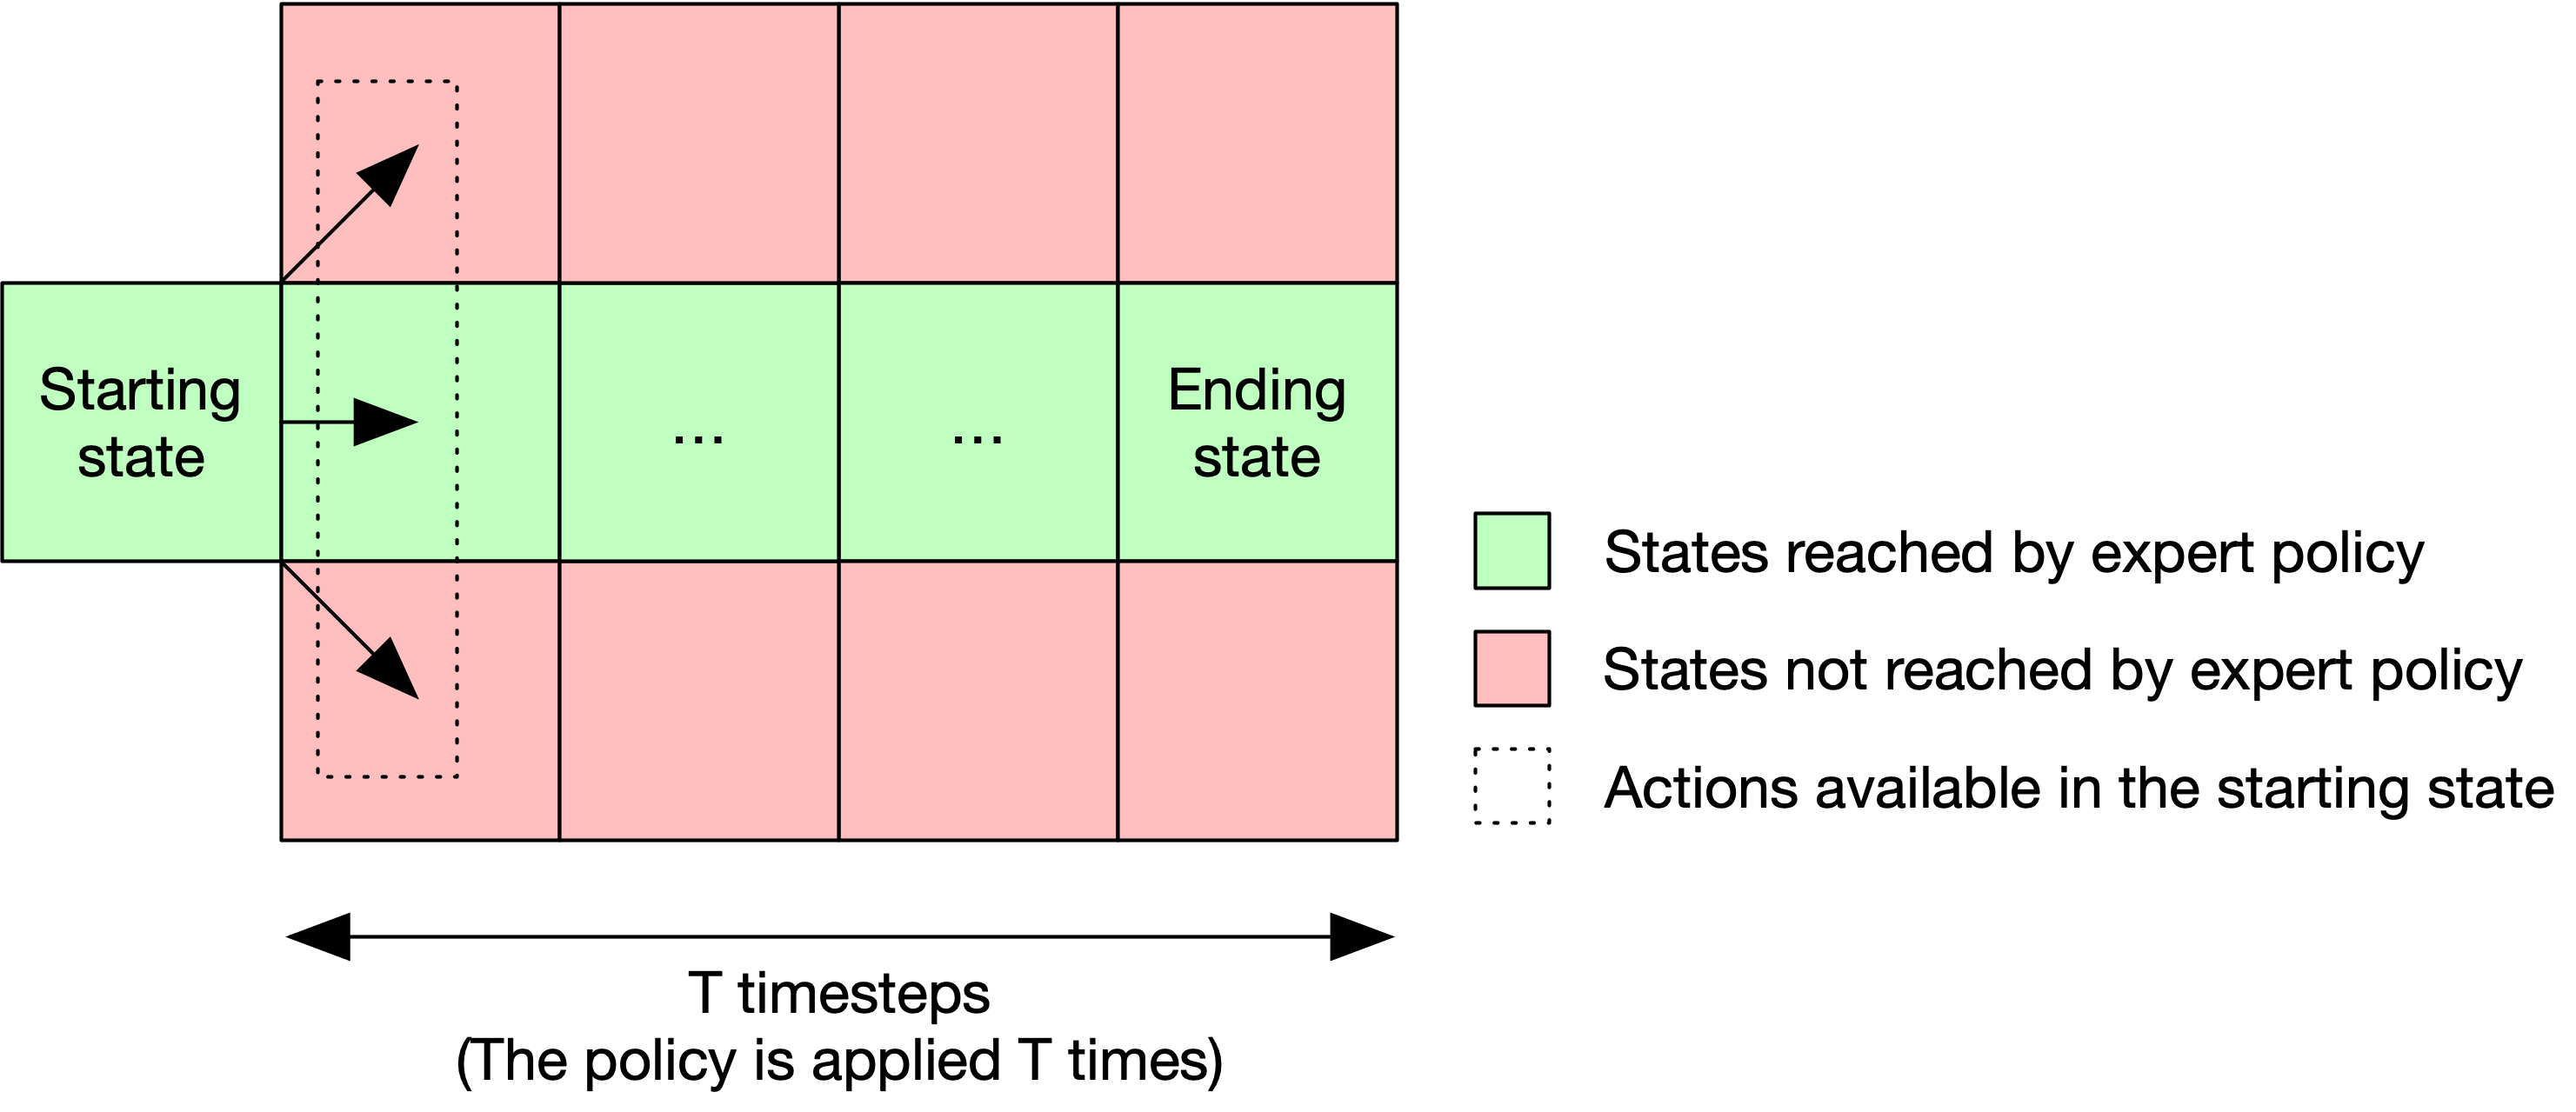
\includegraphics[width=14cm]{tight_rope_diagram}
	\caption{The `tight-rope'' scenario.}
	\label{fig:tight rope}
\end{figure}

\textbf{Supervised learning on expert's policy.} Suppose that an arbitrary path in the tight-rope scenario would involve applying an arbitrary policy $T$ times. Then obviously the expert's path is of length $T$. At each time-step, we treat the expert's state as an training example and the experts' action as the corresponding training label. This one-to-one mapping can be seen as the expert's \textit{policy} - how it reacts (takes actions`) to various (but not all!) situations (states). Aggregating such pairs over all time-steps, we obtain a training set of $T-1$ labeled examples. Finally, we use supervised learning models such as a deep neural network to fit this data. Note that this model then becomes a policy on its own and we denote it by $\pi_{\theta}(\state)$ where $\theta$ parameterizes the model. Importantly, we assume that $\pi_\theta(a \neq \expert(\state) \mid \state) \leq \epsilon$. Note that the entire purpose of $\epsilon$ is to quantify the strength of the supervised learner.

\vspace{1mm}
\textbf{Expected cost of $\pi_{\theta}(\state)$ over $T$ time-step.} The expected cost can be computed intuitively as follows:

$$
\mathbb{E}\left[\sum_{t} c(\state_t, \action_t)\right] \leq
\underbrace{\epsilon T}_{\text{Mistake at }T=1} +
\underbrace{
	(1 - \epsilon)(
		\underbrace{\epsilon (T-1)}_{\text{Mistake at }T=2}
		+
		\underbrace{(1-\epsilon)(\epsilon(T-2)+\cdots)}_{\text{Correct at }T=2}
	)
}_{\text{Correct at }T=1},
$$

assuming that once we make a mistake, we will always be making mistakes since we will be dealing with unseen states. This is, of course, unrealistic in this scenario where there are only 3 actions to choose from (corresponding to the 3 available) states), but this is reasonable as a bound, especially when the state space is large.

\vspace{1mm}

\textbf{Complexity of expected cost.}

\begin{itemize}
	\item T terms because we are making decisions T times (each time we make a decision we create a mistake term)
	\item Each term has $O(\epsilon T)$
	\item total this is $O(\epsilon T^2)$
\end{itemize}

Such a complexity is terrible. 

\section{More general analysis}

Assume $p(\expert(\state) \neq \pi_{\theta}(\state) | \state) \leq \epsilon$. In essence, this assumption assumes that the training of a deep neural network to work decently but makes a small mistake.

\subsection{Case 1: $p_{\text{train}}(\state) \to p_{\theta}(\state)$}

Then at every step, whether we make a mistake, we always land in a state that is available in the training set, so we know how to react. Mention the dagger algorithm.

\subsection{Case 2: $p_{\text{train}}(\state) \neq p_{\theta}(\state)$}

$$
p_{\theta}(\state_t) = 
\underbrace{(1-\epsilon)^t}_{\text{0 mistake}} p_{\text{train}} (\state_t) 
+ 
\underbrace{(1 - (1 - \epsilon)^t)}_{\geq 1 \text{ mistakes}} p_{\text{mistake}}(\state_t)
$$

\begin{itemize}
	\item no mistake wrt to the expert, in this case, still in the training distribution
	\item made at least one mistake, not sure where it is now; note that since p train and p mistake are probability distributions so they might overlap, we can't really be sure about this (how well the neural net generalize)
\end{itemize}

We can use the equation above to prove that (this will help us later in proving the bound):

$$
\sum_{\state_t} \left|p_{\theta}\left(\mathbf{s}_{t}\right)-p_{\text {train}}\left(\mathbf{s}_{t}\right)\right|=\left(1-(1-\epsilon)^{t}\right)
\sum_{\state_t}\left|p_{\text{mistake}}\left(\mathbf{s}_{t}\right)-p_{\text {train}}\left(\mathbf{s}_{t}\right)\right|
$$

where the absolute value operator denotes the \textit{total variation divergence} between two distributions (review).

because 

\begin{align*}
&\sum_{\state_t} \left| p_{\theta}\left(\mathbf{s}_{t}\right)-p_{\text {train}}\left(\mathbf{s}_{t}\right)  \right| \\
=&
\sum_{\state_t}
\left| 
(1-\epsilon)^t p_{\text{train}} (\state_t) + 
(1 - (1 - \epsilon)^t) p_{\text{mistake}}(\state_t) -
(1-\epsilon)^t p_{\text{train}} (\state_t) - 
(1 - (1 - \epsilon)^t) p_{\text{train}}(\state_t) 
\right|
\\
=& 
\sum_{\state_t}
\left|
\underbrace{(1 - (1 - \epsilon)^t)}_{\text{Positive}} p_{\text{mistake}}(\state_t) -
(1 - (1 - \epsilon)^t) p_{\text{train}}(\state_t)
\right|
\\
=& 
(1 - (1 - \epsilon)^t) 
\underbrace{
\sum_{\state_t}
\left|
p_{\text{mistake}}(\state_t) - p_{\text{train}}(\state_t)
\right|
}_{\leq 2}
\\
\leq& 2 (1 - (1 - \epsilon)^t) 
\\
\leq& 2 \epsilon t \tag*{Using the inequality that $(1-\epsilon)^t \geq 1 - \epsilon t$ for $\epsilon \in [0, 1]$}
\end{align*}

\begin{align*}
\mathbb{E}_{\tau \sim p(\tau)}\left[\sum_{t} c_t(\state_t, \action_t)\right] 
&= \sum_t \mathbb{E}_{\state_t \sim p_{\theta}(\state_t)} \left[ c_t(\state_t, \action_t) \right] \tag*{By the linearity of expectations ...} \\
&= \sum_t \sum_{\state_t} p_{\theta}(\state_t) c_t(\state_t, \action_t) \\
&= \sum_t \sum_{\state_t} \{p_{\text{train}}(\state_t) + p_{\theta}(\state_t) - p_{\text{train}}(\state_t)\} c_t(\state_t, \action_t) \\
&= \sum_t \sum_{\state_t} p_{\text{train}}(\state_t) c_t(\state_t, \action_t) +
\{p_{\theta}(\state_t) - p_{\text{train}}(\state_t)\} c_t(\state_t, \action_t)\\
&\leq \sum_t \sum_{\state_t} p_{\text{train}}(\state_t) c_t(\state_t, \action_t) +
\left| p_{\theta}(\state_t) - p_{\text{train}}(\state_t)\right| c_t(\state_t, \action_t)\\
&\leq \sum_t \sum_{\state_t} p_{\text{train}}(\state_t) c_t(\state_t, \action_t) +
\left| p_{\theta}(\state_t) - p_{\text{train}}(\state_t)\right| c_{\max}\\
&\leq \sum_t \sum_{\state_t} p_{\text{train}}(\state_t) c_t(\state_t, \action_t) +
\left| p_{\theta}(\state_t) - p_{\text{train}}(\state_t)\right| \tag*{$c_{\max}=1$ because we are using the zero-one loss}\\ 
&= \sum_t \epsilon + 2\epsilon t
\end{align*} 

where $\tau = \{ \state_1, \action_1, \cdots, \state_t, \action_t\}$ is a sampled trajectory

\section{Questions}

\begin{itemize}
	\item What does it mean to subtract two distributions
\end{itemize}

\end{document}
